\chapter{結論}
\label{chap:conclusion}

この章では本研究における結論について述べる.
まず今後の展望について述べ, 次に具体的なデータの収集・活用方法について述べる,
最後に本研究のまとめを行い,卒業論文とする.

\section{今後の展望}
第\ref{chap:main_experiment}章の評価実験において, 人は一度顔の筋肉を弛緩してから笑顔になるユーザーに対して嗜好傾向がある可能性を示した.
しかし, 本研究では被験者41人, 有効データ36個と非常に傾向分析には少ないデータとなっている.
さらに, データの大半は20代および男性のデータが約68\%と偏りのあるデータとなっている.
今後, 追加データを取得する際には設置場所を考慮し,バランスのとれたデータを取得する必要がある.
また, 本研究は表情ベースでの判断のみになってしまっており, ここの内面状態やどのような基準で
順位づけを行っているのかを考慮することができていない.
Open Research Forum においてユーザー1人,1人へインタビュー調査を行うことは叶わなかったため,
今後は表情ベースの判断に加え, 内面的状態を考慮してデータを提案することが可能なシステム
構成を考える必要がある.

\subsection{TEAM Smileとの連携}
私は慶應義塾大学湘南藤沢キャンパス中澤仁研究室が関与している健康情報コンソーシアムの中にある
Team SMILEに参加し, SmileMeterの開発に携わっている.\cite{teamSMILE}SmileMeterとは自分の笑顔状態を把握し,
自分で安全に保存・蓄積できる、素敵なキオスクデバイスである.
今までに玉川高島屋や, イオンモール幕張新都心, 地域のイベントなどに出展をし,
笑顔と健康の大切さを伝える活動を行っている.
今後,TeamSmileの活動が発展していく上でより多く, 精度の高いデータを集取し活動に活かすために
本システムで作成したOpenFaceを使用した表情解析モジュールをSmileMeterに組み込む予定である.
実証実験の場が今後増えていき, より多くのデータを取得することが見込まれる.
本研究では40人といった小規模実験を行ったが,  より多く幅広い年齢・性別のデータを分析することで
より人と人とを繋ぐシステムを構築するためのデータを取得する.

\begin{figure}[htbp]
    \begin{center}
       \fbox{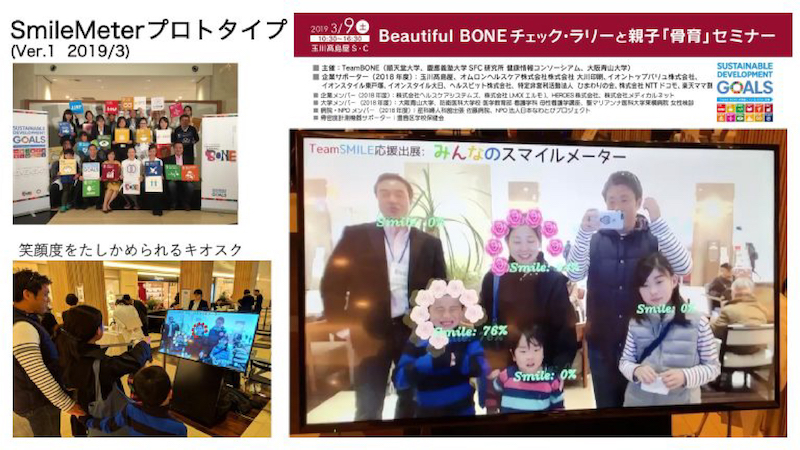
\includegraphics[width=150mm,bb=0 0 800 450]{takashimaya.jpg}}
    \end{center}
    \caption{玉川高島屋の出展}
    \label{fig:takashimaya}
\end{figure}

\begin{figure}[htbp]
    \begin{center}
       \fbox{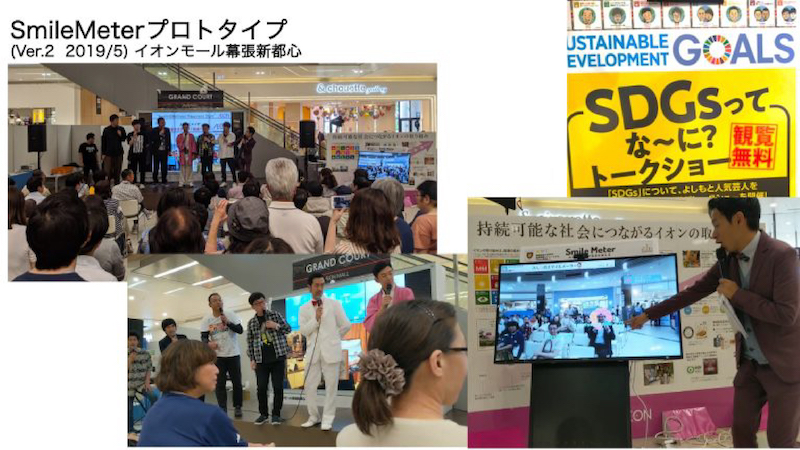
\includegraphics[width=150mm,bb=0 0 800 450]{aeon.jpg}}
    \end{center}
    \caption{イオンモール幕張新都心の出展}
    \label{fig:aeon}
\end{figure}

\begin{figure}[htbp]
    \begin{center}
       \fbox{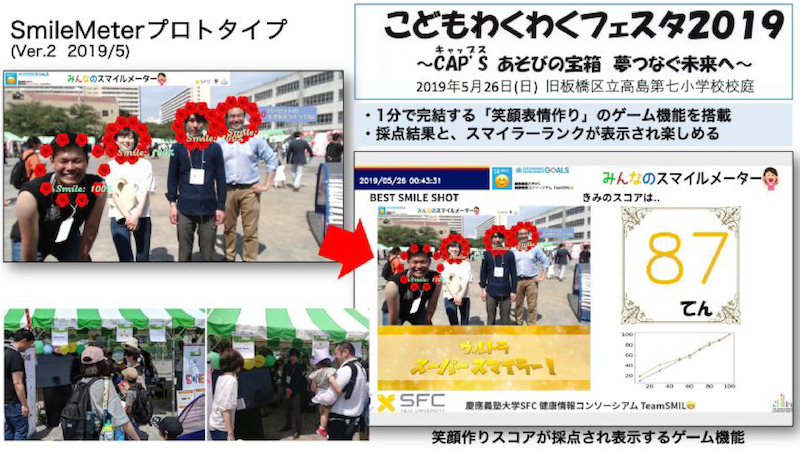
\includegraphics[width=150mm,bb=0 0 800 450]{itabashi.jpg}}
    \end{center}
    \caption{板橋区イベントの出展}
    \label{fig:itabashi}
\end{figure}

\subsection{1月下旬に行った実証実験について}
TeamSMILEの共同研究をしている福岡の株式会社LMOの九州良縁フェスティバルに2020年1月18日鹿児島,
19日熊本に参加した. 本イベントは, 20代以上の独身男女が参加する結婚活動イベントであり,
TeamSMILEはSmileMeterを展示し,来場者にむけて実証実験を行った.
将来のパートナーを決める際には, 自分の運命を大きく作用するため相手選びがより慎重になる.
重要な選択をする際に, 自身や相手の根本的な部分を表情によって分析し, 情報提供をすることができれば
より自分にも相手にとっても良好な人間関係の構築をすることが可能になる.
実際に, SmileMeterを体験したカップルには笑顔が増えシステムがお互いにコミュニケーションの
きっかけとなるような働きをしているように思われた.
今後, 本システムの表情解析モジュールを導入し, 良縁な関係を築いていくきっかけになる,
そしてユーザーごとの引き合わせをすることができるシステムの構築を将来的な展望とする.

\begin{figure}[htbp]
    \begin{center}
       \fbox{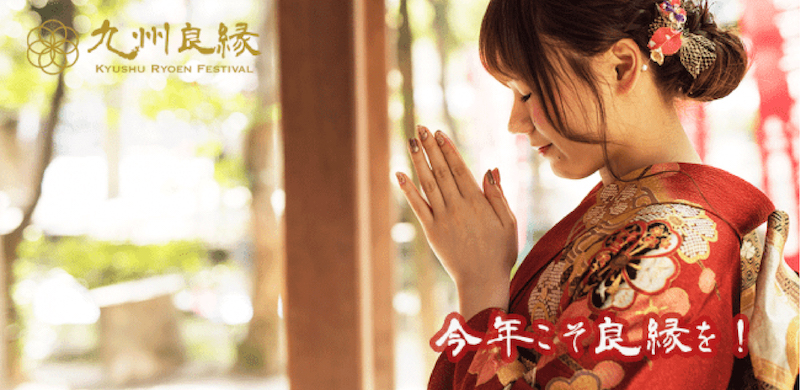
\includegraphics[width=150mm,bb=0 0 800 390]{lmo.jpg}}
    \end{center}
    \caption{株式会社LMOとの共同イベント}
    \label{fig:lmo}
\end{figure}

\begin{figure}[htbp]
    \begin{center}
       \fbox{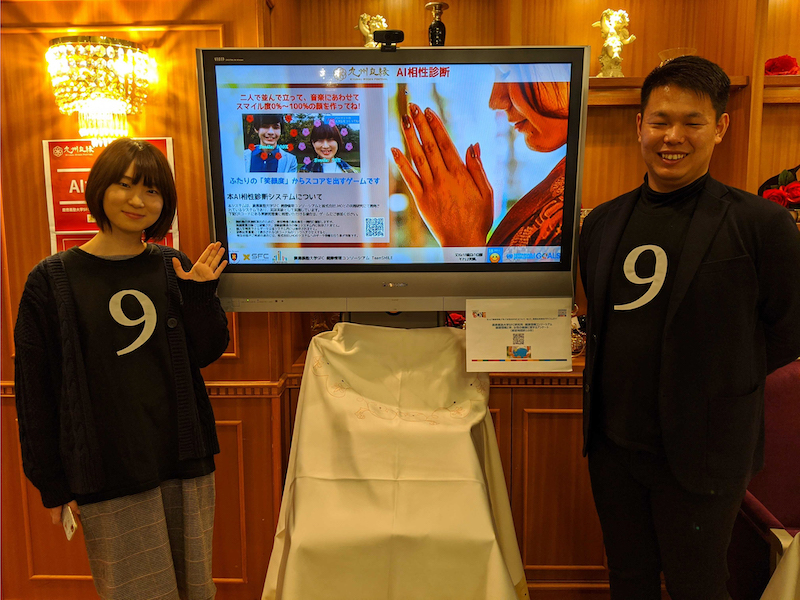
\includegraphics[width=150mm,bb=0 0 800 600]{kyushu.jpg}}
    \end{center}
    \caption{株式会社LMOとの共同イベント当日}
    \label{fig:kyushu}
\end{figure}

\section{本論文まとめ}
本研究は自身の笑顔の作り方と表情ベースによる嗜好判断分析を行った.
41人に対して, 36個の有効笑顔動画データおよびFAU値を取得することができた.
取得したデータの分析により, 人は一度表情の筋肉を弛緩してから笑顔になる笑い方に惹かれている
傾向がみられた.
本システムはより多くのデータを収集, ユーザーの内面状態を組み込むことで
仕事または結婚時のパートナー選択に有益な情報を提供することが可能である.
情報過多になっている現代社会において, ユーザーにとって適切なデータ提供を行い,
より良い人間関係の構築をする機会を提供することが可能になると考えられる.
今後, TeamSmileの活動等を通じて多くのデータを取得し,
本研究, 本システムが人と人とを繋ぐ役割を担うようなシステムになることを期待して卒業論文とする.
